\documentclass{ximera}

%\usepackage{todonotes}

\newcommand{\todo}{}

\usepackage{esint} % for \oiint
\ifxake%%https://math.meta.stackexchange.com/questions/9973/how-do-you-render-a-closed-surface-double-integral
\renewcommand{\oiint}{{\large\bigcirc}\kern-1.56em\iint}
\fi


\graphicspath{
  {./}
  {ximeraTutorial/}
  {basicPhilosophy/}
  {functionsOfSeveralVariables/}
  {normalVectors/}
  {lagrangeMultipliers/}
  {vectorFields/}
  {greensTheorem/}
  {shapeOfThingsToCome/}
  {dotProducts/}
  {partialDerivativesAndTheGradientVector/}
  {../productAndQuotientRules/exercises/}
  {../normalVectors/exercisesParametricPlots/}
  {../continuityOfFunctionsOfSeveralVariables/exercises/}
  {../partialDerivativesAndTheGradientVector/exercises/}
  {../directionalDerivativeAndChainRule/exercises/}
  {../commonCoordinates/exercisesCylindricalCoordinates/}
  {../commonCoordinates/exercisesSphericalCoordinates/}
  {../greensTheorem/exercisesCurlAndLineIntegrals/}
  {../greensTheorem/exercisesDivergenceAndLineIntegrals/}
  {../shapeOfThingsToCome/exercisesDivergenceTheorem/}
  {../greensTheorem/}
  {../shapeOfThingsToCome/}
  {../separableDifferentialEquations/exercises/}
  {vectorFields/}
}

\newcommand{\mooculus}{\textsf{\textbf{MOOC}\textnormal{\textsf{ULUS}}}}

\usepackage{tkz-euclide}
\usepackage{tikz}
\usepackage{tikz-cd}
\usetikzlibrary{arrows}
\tikzset{>=stealth,commutative diagrams/.cd,
  arrow style=tikz,diagrams={>=stealth}} %% cool arrow head
\tikzset{shorten <>/.style={ shorten >=#1, shorten <=#1 } } %% allows shorter vectors

\usetikzlibrary{backgrounds} %% for boxes around graphs
\usetikzlibrary{shapes,positioning}  %% Clouds and stars
\usetikzlibrary{matrix} %% for matrix
\usepgfplotslibrary{polar} %% for polar plots
\usepgfplotslibrary{fillbetween} %% to shade area between curves in TikZ
%\usetkzobj{all}
\usepackage[makeroom]{cancel} %% for strike outs
%\usepackage{mathtools} %% for pretty underbrace % Breaks Ximera
%\usepackage{multicol}
\usepackage{pgffor} %% required for integral for loops



%% http://tex.stackexchange.com/questions/66490/drawing-a-tikz-arc-specifying-the-center
%% Draws beach ball
\tikzset{pics/carc/.style args={#1:#2:#3}{code={\draw[pic actions] (#1:#3) arc(#1:#2:#3);}}}



\usepackage{array}
\setlength{\extrarowheight}{+.1cm}
\newdimen\digitwidth
\settowidth\digitwidth{9}
\def\divrule#1#2{
\noalign{\moveright#1\digitwidth
\vbox{\hrule width#2\digitwidth}}}




% \newcommand{\RR}{\mathbb R}
% \newcommand{\R}{\mathbb R}
% \newcommand{\N}{\mathbb N}
% \newcommand{\Z}{\mathbb Z}

\newcommand{\sagemath}{\textsf{SageMath}}


%\renewcommand{\d}{\,d\!}
%\renewcommand{\d}{\mathop{}\!d}
%\newcommand{\dd}[2][]{\frac{\d #1}{\d #2}}
%\newcommand{\pp}[2][]{\frac{\partial #1}{\partial #2}}
% \renewcommand{\l}{\ell}
%\newcommand{\ddx}{\frac{d}{\d x}}

% \newcommand{\zeroOverZero}{\ensuremath{\boldsymbol{\tfrac{0}{0}}}}
%\newcommand{\inftyOverInfty}{\ensuremath{\boldsymbol{\tfrac{\infty}{\infty}}}}
%\newcommand{\zeroOverInfty}{\ensuremath{\boldsymbol{\tfrac{0}{\infty}}}}
%\newcommand{\zeroTimesInfty}{\ensuremath{\small\boldsymbol{0\cdot \infty}}}
%\newcommand{\inftyMinusInfty}{\ensuremath{\small\boldsymbol{\infty - \infty}}}
%\newcommand{\oneToInfty}{\ensuremath{\boldsymbol{1^\infty}}}
%\newcommand{\zeroToZero}{\ensuremath{\boldsymbol{0^0}}}
%\newcommand{\inftyToZero}{\ensuremath{\boldsymbol{\infty^0}}}



% \newcommand{\numOverZero}{\ensuremath{\boldsymbol{\tfrac{\#}{0}}}}
% \newcommand{\dfn}{\textbf}
% \newcommand{\unit}{\,\mathrm}
% \newcommand{\unit}{\mathop{}\!\mathrm}
% \newcommand{\eval}[1]{\bigg[ #1 \bigg]}
% \newcommand{\seq}[1]{\left( #1 \right)}
% \renewcommand{\epsilon}{\varepsilon}
% \renewcommand{\phi}{\varphi}


% \renewcommand{\iff}{\Leftrightarrow}

% \DeclareMathOperator{\arccot}{arccot}
% \DeclareMathOperator{\arcsec}{arcsec}
% \DeclareMathOperator{\arccsc}{arccsc}
% \DeclareMathOperator{\si}{Si}
% \DeclareMathOperator{\scal}{scal}
% \DeclareMathOperator{\sign}{sign}


%% \newcommand{\tightoverset}[2]{% for arrow vec
%%   \mathop{#2}\limits^{\vbox to -.5ex{\kern-0.75ex\hbox{$#1$}\vss}}}
% \newcommand{\arrowvec}[1]{{\overset{\rightharpoonup}{#1}}}
% \renewcommand{\vec}[1]{\arrowvec{\mathbf{#1}}}
% \renewcommand{\vec}[1]{{\overset{\boldsymbol{\rightharpoonup}}{\mathbf{#1}}}}

% \newcommand{\point}[1]{\left(#1\right)} %this allows \vector{ to be changed to \vector{ with a quick find and replace
% \newcommand{\pt}[1]{\mathbf{#1}} %this allows \vec{ to be changed to \vec{ with a quick find and replace
% \newcommand{\Lim}[2]{\lim_{\point{#1} \to \point{#2}}} %Bart, I changed this to point since I want to use it.  It runs through both of the exercise and exerciseE files in limits section, which is why it was in each document to start with.

% \DeclareMathOperator{\proj}{\mathbf{proj}}
% \newcommand{\veci}{{\boldsymbol{\hat{\imath}}}}
% \newcommand{\vecj}{{\boldsymbol{\hat{\jmath}}}}
% \newcommand{\veck}{{\boldsymbol{\hat{k}}}}
% \newcommand{\vecl}{\vec{\boldsymbol{\l}}}
% \newcommand{\uvec}[1]{\mathbf{\hat{#1}}}
% \newcommand{\utan}{\mathbf{\hat{t}}}
% \newcommand{\unormal}{\mathbf{\hat{n}}}
% \newcommand{\ubinormal}{\mathbf{\hat{b}}}

% \newcommand{\dotp}{\bullet}
% \newcommand{\cross}{\boldsymbol\times}
% \newcommand{\grad}{\boldsymbol\nabla}
% \newcommand{\divergence}{\grad\dotp}
% \newcommand{\curl}{\grad\cross}
%\DeclareMathOperator{\divergence}{divergence}
%\DeclareMathOperator{\curl}[1]{\grad\cross #1}
% \newcommand{\lto}{\mathop{\longrightarrow\,}\limits}

% \renewcommand{\bar}{\overline}

\colorlet{textColor}{black}
\colorlet{background}{white}
\colorlet{penColor}{blue!50!black} % Color of a curve in a plot
\colorlet{penColor2}{red!50!black}% Color of a curve in a plot
\colorlet{penColor3}{red!50!blue} % Color of a curve in a plot
\colorlet{penColor4}{green!50!black} % Color of a curve in a plot
\colorlet{penColor5}{orange!80!black} % Color of a curve in a plot
\colorlet{penColor6}{yellow!70!black} % Color of a curve in a plot
\colorlet{fill1}{penColor!20} % Color of fill in a plot
\colorlet{fill2}{penColor2!20} % Color of fill in a plot
\colorlet{fillp}{fill1} % Color of positive area
\colorlet{filln}{penColor2!20} % Color of negative area
\colorlet{fill3}{penColor3!20} % Fill
\colorlet{fill4}{penColor4!20} % Fill
\colorlet{fill5}{penColor5!20} % Fill
\colorlet{gridColor}{gray!50} % Color of grid in a plot

\newcommand{\surfaceColor}{violet}
\newcommand{\surfaceColorTwo}{redyellow}
\newcommand{\sliceColor}{greenyellow}




\pgfmathdeclarefunction{gauss}{2}{% gives gaussian
  \pgfmathparse{1/(#2*sqrt(2*pi))*exp(-((x-#1)^2)/(2*#2^2))}%
}


%%%%%%%%%%%%%
%% Vectors
%%%%%%%%%%%%%

%% Simple horiz vectors
\renewcommand{\vector}[1]{\left\langle #1\right\rangle}


%% %% Complex Horiz Vectors with angle brackets
%% \makeatletter
%% \renewcommand{\vector}[2][ , ]{\left\langle%
%%   \def\nextitem{\def\nextitem{#1}}%
%%   \@for \el:=#2\do{\nextitem\el}\right\rangle%
%% }
%% \makeatother

%% %% Vertical Vectors
%% \def\vector#1{\begin{bmatrix}\vecListA#1,,\end{bmatrix}}
%% \def\vecListA#1,{\if,#1,\else #1\cr \expandafter \vecListA \fi}

%%%%%%%%%%%%%
%% End of vectors
%%%%%%%%%%%%%

%\newcommand{\fullwidth}{}
%\newcommand{\normalwidth}{}



%% makes a snazzy t-chart for evaluating functions
%\newenvironment{tchart}{\rowcolors{2}{}{background!90!textColor}\array}{\endarray}

%%This is to help with formatting on future title pages.
\newenvironment{sectionOutcomes}{}{}



%% Flowchart stuff
%\tikzstyle{startstop} = [rectangle, rounded corners, minimum width=3cm, minimum height=1cm,text centered, draw=black]
%\tikzstyle{question} = [rectangle, minimum width=3cm, minimum height=1cm, text centered, draw=black]
%\tikzstyle{decision} = [trapezium, trapezium left angle=70, trapezium right angle=110, minimum width=3cm, minimum height=1cm, text centered, draw=black]
%\tikzstyle{question} = [rectangle, rounded corners, minimum width=3cm, minimum height=1cm,text centered, draw=black]
%\tikzstyle{process} = [rectangle, minimum width=3cm, minimum height=1cm, text centered, draw=black]
%\tikzstyle{decision} = [trapezium, trapezium left angle=70, trapezium right angle=110, minimum width=3cm, minimum height=1cm, text centered, draw=black]


\title{Dominance}

\begin{document}

\begin{abstract}
relatively bigger
\end{abstract}
\maketitle







\textbf{\textcolor{red!70!black}{$\rhd$}} Do functions tend to infinity differently? \\



For example,

Both $p(x) = 6x^3 - 5x + 2$ and $w(t) = 2t^2 = 4t - 5$ approach $\infty$ as you move further out in the domain.



\[    \lim_{x \to \infty} p(x) = \infty  \, \text{ and }  \,       \lim_{t \to \infty} w(t) = \infty                \]

\textbf{\textcolor{blue!55!black}{$\blacktriangleright$}} Do they approach $\infty$ in the same way? 

\textbf{\textcolor{blue!55!black}{$\blacktriangleright$}} What do we mean by ``same way''?  \\



How should we compare $p(x)$ and $w(t)$ to decide if they approach $\infty$ in the same way?  \\


We have two ways of comparing things: differences and quotients. \\

Quotients work better for comparing the end-behavior of functions. \\


By the ``same way'', we are picturing a horizontal asymptote, like for rational functions. This occurs when the degrees of the polynomials are equal.   The polynomial in the numerator and the polynomial in the denominator ``behave in the same way'' as we move far out in the domain.  The two polynomials are somehow ``at the same level'' of infinity. \\







\begin{idea}


To decide if two functions, $f$ and $g$, approach infinity in the same way, 

\begin{enumerate}
\item create a quotient: $\frac{f(x)}{g(x)}$ \\


\item examine the end-behavior of this quotient: $\lim\limits_{x \to \infty} \frac{f(x)}{g(x)}$ \\


\item if this limit equals a nonzero constant, then $f$ and $g$ approach $\infty$ the same - neither overshadows the other.
\end{enumerate}


If the limit is $1$, then people sometimes say the two functions are asymptotically equivalent. People sometimes use the symbol $\sim$ for asymptotically equivalent. \\

\end{idea}




\begin{center}

\textbf{\textcolor{purple!85!blue}{Perhaps more important for future Calculus courses is when this limit is $0$.}} \\

\end{center}















\section*{Dominance}



\begin{definition}  \textbf{\textcolor{green!50!black}{Dominance}} 

If the quotient limit equals $0$,

\[  \lim_{x \to \infty} \frac{f(x)}{g(x)}  = 0\]

then we say that $g$ \textbf{dominates} $f$. \\



Sometimes people use a double inequality for dominates:  $f \ll g$.\\

\end{definition}



When one function dominates another, then it approaches infinity in such a way that the other function is like $0$ in comparison. When the dominate function is the denominator, then this drives the quotient to $0$.


Our initial order of dominance looks like this. \\


\begin{summary} \textbf{\textcolor{purple!85!blue}{Order of Dominance}}


When we are comparing \textbf{unbounded} function values, then \\

\[   bounded functions (constants, \, sine, \, cosine)  \ll logarithmic \ll power (polynomial) \ll  exponential  \]



This goes for their powers as well. 


\[   bounded functions (constants, \, sine, \, cosine)  \ll logarithmic^{power} \ll power polynomial^{power} \ll  exponential  \]



\end{summary}

\textbf{Note:} power functions include roots and radicals and linear and polynomials.










\begin{example} Dominance


Let $g(x) = \frac{\ln(x)}{x}$.

Graph of $y = g(x)$.


According to our order of dominance, the denominator is a linear function and should dominate the numerator function, which is a logarithm.  Therefore, as $x$ approach infinity, this whole fraction should approach $0$.


\begin{image}
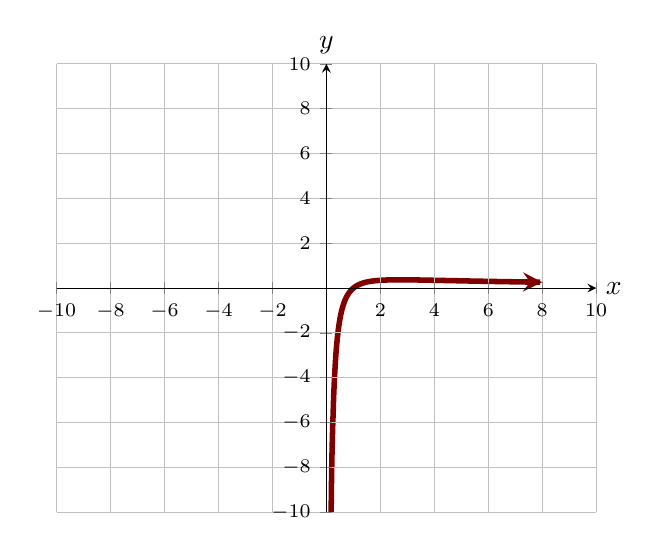
\begin{tikzpicture}
  \begin{axis}[
            domain=-10:10, ymax=10, xmax=10, ymin=-10, xmin=-10,
            axis lines =center, xlabel=$x$, ylabel=$y$, grid = major,
            ytick={-10,-8,-6,-4,-2,2,4,6,8,10},
            xtick={-10,-8,-6,-4,-2,2,4,6,8,10},
            yticklabels={$-10$,$-8$,$-6$,$-4$,$-2$,$2$,$4$,$6$,$8$,$10$}, 
            xticklabels={$-10$,$-8$,$-6$,$-4$,$-2$,$2$,$4$,$6$,$8$,$10$},
            ticklabel style={font=\scriptsize},
            every axis y label/.style={at=(current axis.above origin),anchor=south},
            every axis x label/.style={at=(current axis.right of origin),anchor=west},
            axis on top
          ]
          

            \addplot [line width=2, penColor2, smooth,samples=100,domain=(0.1:8), <->] {ln(x)/x};


  \end{axis}
\end{tikzpicture}
\end{image}



Let's zoom in.


\begin{center}
\desmos{3dmdtmts1h}{400}{300}
\end{center}



Here we can see the graph peak and begin to come back down.   \\


However, we are investigating \textbf{end-behavior}.  $18$ is not very large. We are interested in the values of $g(x)$ when $x$ is very very large. \\  

That was not a good graph for our purposes.  We are interested in large values of $x$.









\begin{image}
\begin{tikzpicture}
  \begin{axis}[
            domain=-1:1000, ymax=0.75, xmax=1000, ymin=-1, xmin=-1,
            axis lines =center, xlabel=$x$, ylabel={$y=g(x)$}, 
            ytick={0.5},
            xtick={200,400,600,800},
            xticklabels={$200$,$400$,$600$,$800$},
            ticklabel style={font=\scriptsize},
            every axis y label/.style={at=(current axis.above origin),anchor=south},
            every axis x label/.style={at=(current axis.right of origin),anchor=west},
            axis on top
          ]
          

            \addplot [line width=2, penColor2, smooth,samples=100,domain=(1:950), <->] {ln(x)/x};




           

  \end{axis}
\end{tikzpicture}
\end{image}






Eventually, the graph approaches the x-axis as the function value approaches $0$. \\


The denominator function, $x$, dominates the numerator function, $\ln(x)$.   The values of $\ln(x)$ become like $0$ compared to the values of $x$, when $x$ is very very very large. Not when $x$ takes on small values.  Not when $x$ has medium values.  Dominance is a statement when $x$ takes on very very very large values.




\end{example}







The level of dominance includes powers.  We can raise the power of $\ln(x)$, but they are still overshadowed by values of $x$, when $x$ is very very very large. \\

















\begin{example} Powers


Graph of $y = \frac{(\ln(x))^5}{x}$.

$x$ should dominate any power of $\ln(x)$.  Therefore, the graph of this function should eventually aproach the the $x$-axis as the function value approaches $0$. \\


If this function approaches $0$, then it must get below and stay below $2$, eventually. How far out in the domain do you need to go before this function eventually dips and stays below $2$.


\begin{center}
\desmos{rksndotdsv}{400}{300}
\end{center}




\textbf{Hint:} Look out around $1,000,000$.

\end{example}







For the following limits, refer to our order of dominance.

\begin{question}

\[
\lim\limits_{t \to \infty} \frac{x^6}{e^x} = \answer{0}
\]

\end{question}









\begin{question}

\[
\lim\limits_{\theta \to \infty} \frac{\cos(2 \theta)}{\ln(\theta)} = \answer{0}
\]

\end{question}









\begin{question}

\[
\lim\limits_{y \to \infty} \frac{y^{1345}}{2^y} = \answer{0}
\]

\end{question}












\begin{question}

\[
\lim\limits_{w \to \infty} \frac{(\ln(w))^{78}}{w} = \answer{0}
\]

\end{question}






\begin{idea} \textbf{\textcolor{blue!55!black}{Upsidedown}}


When we talk about dominance, we phrase it in terms of approaching $0$.  The quotient might be approaching $0$ through psitive numbers or negative numbers.  It doesn't matter because $-0 = 0$.


If we our quotient is upsidedown and the dominate function is in the numerator, then we also need to think about the sign.


\end{idea}



\begin{example}




\[
\lim\limits_{k \to \infty} \frac{8}{3^k} = 0
\]



\[
\lim\limits_{k \to \infty} \frac{3^k}{8} = \infty 
\]




\end{example}









\begin{example}



Since $4 - k \ll 3^k$,

\[
\lim\limits_{k \to \infty} \frac{4 - k}{3^k} = 0
\]


When thinking about the reciprocal, then we need to keep in mind that $4 - k < 0$ for large positive values of $k$.



\[
\lim\limits_{k \to \infty} \frac{3^k}{4 - k} = -\infty 
\]




\end{example}






\subsection*{Sums and Differences}


Dominance also helps us identify the most important terms in a function's formula.


When one term in a formula dominates over an added term, then we can remove the dominated term from our analysis. \\






\begin{example}

Consider the function $B(t) = \frac{3e^t - 5}{e^t + 1}$. \\


$\blacktriangleright$ As $t \to \infty$, $3e^t$ dominates $-5$. \\

$\blacktriangleright$ As $t \to \infty$, $3^t$ dominates $1$. \\




As $t \to \infty$, the exponential pieces will dominate the constant pieces in each expression.  

\[   B(t) = \frac{3e^t - 5}{e^t + 1} \sim \frac{3 e^t}{e^t} = 3   \]




\textbf{\textcolor{blue!55!black}{$\blacktriangleright$}} Now consider the other direction. \\


As $t \to -\infty$, we have a different story.   



\[   \lim\limits_{t \to -\infty} 3 e^t  = 0  \]


This reverses the dominance.


\[   \lim\limits_{t \to -\infty} \frac{e^t}{5} = 0   \]



As $t \to -\infty$, we have a different story.  $\lim\limits_{t \to -\infty} e^t = 0$. Therefore, in this case, the constant terms dominate.


\[   B(t) = \frac{3e^t - 5}{e^t + 1} \sim \frac{-5}{1} = -5   \]








\end{example}




\begin{idea} \textbf{\textcolor{blue!55!black}{Limiting Behavior}}



If $f(x) \ll g(x)$, then $f(x) + g(x) \sim g(x)$



\end{idea}


This helps us think about limiting behavior.



\begin{example}


\[
\lim\limits_{x \to -\infty} \frac{e^{x} + 5x^2 + \sqrt{4-x} - 7}{5 + 6x^4 + e^{-x}} = \lim\limits_{x \to -\infty} \frac{5x^2}{e^{-x}} = 0
\]



\end{example}







\begin{example}


\[
\lim\limits_{x \to \infty} \frac{\sqrt{x^3 - x + 1}}{x \, \sqrt{2 \, x-6}} = \lim\limits_{x \to \infty} \frac{\sqrt{x^3}}{x \, \sqrt{2 \, x}} = \lim\limits_{x \to \infty} \frac{x \, \sqrt{x}}{x \, \sqrt{x} \, \sqrt{2} } = \lim\limits_{x \to \infty} \frac{1}{\sqrt{2} } = \frac{1}{\sqrt{2} }
\]



\end{example}













\begin{center}
\textbf{\textcolor{green!50!black}{ooooo-=-=-=-ooOoo-=-=-=-ooooo}} \\

more examples can be found by following this link\\ \link[More Examples of Dominance]{https://ximera.osu.edu/csccmathematics/precalculus1/precalculus1/functionComparison/examples/exampleList}

\end{center}








\end{document}
